% =====================================================================
%  Bachelor thesis, Tarik Akinci
%  Build: latexmk (LaTeX Workshop in VS Code does this on save).
%  Engine: pdflatex + biber. Output goes to thesis/build/.
%
%  Where things are:
%    preamble.tex            packages, macros (\fillin, \src, \todo, \llama, ...)
%    frontmatter/            title page, declaration, abstract
%    sections/               one file per section, in reading order
%    appendix/               appendix sections
%    references.bib          bibliography (entries marked VERIFY need checking)
%    figures/                put new thesis figures here
%
%  Structure follows reports/proposal_sketch.md (abstract, introduction
%  P1-P5, RQs, contributions, method, evidence, limits), expanded into the
%  usual paper layout and the outline in CLAUDE.md section 10.
% =====================================================================
\documentclass[11pt,a4paper]{article}
% =====================================================================
%  preamble.tex : packages, layout, macros
%  You should rarely need to touch this file.
% =====================================================================

% ---------- draft / final switch ------------------------------------
% \drafttrue  : TODO notes and source pointers are shown in the margin
% \draftfalse : everything disappears, ready for submission
\newif\ifdraft
\drafttrue

% ---------- fonts and encoding --------------------------------------
\usepackage[T1]{fontenc}
\usepackage{newtxtext,newtxmath}   % Times-like text and maths (as in ACL papers)
\usepackage[english]{babel}
\usepackage{microtype}
\usepackage{csquotes}

% ---------- page layout ---------------------------------------------
\usepackage[a4paper,margin=2.5cm,marginparwidth=2cm]{geometry}
\usepackage{setspace}
\onehalfspacing                     % common for theses; use \singlespacing for paper look
\usepackage{parskip}                % paragraphs separated by space, no indent
\setlength{\parskip}{0.6em}

% ---------- maths, tables, figures ----------------------------------
\usepackage{amsmath}
\usepackage{bm}
\usepackage{booktabs}               % \toprule \midrule \bottomrule
\usepackage{tabularx}
\usepackage{multirow}
\usepackage{threeparttable}         % table notes
\usepackage[group-separator={,},group-minimum-digits=4]{siunitx}
\usepackage{graphicx}
\graphicspath{{figures/}{../D3code-main/scripts/figures/}}
\usepackage{caption}
\usepackage{subcaption}
\captionsetup{font=small,labelfont=bf}
\usepackage{float}
\usepackage{enumitem}
\setlist{itemsep=0.2em,topsep=0.3em}
\usepackage{xcolor}
\usepackage[most]{tcolorbox}        % prompt boxes

% ---------- bibliography (biblatex + biber, author-year) ------------
\usepackage[backend=biber,
            style=authoryear,
            natbib=true,             % \citet{} = Author (Year), \citep{} = (Author, Year)
            maxcitenames=2,
            maxbibnames=10,
            uniquelist=false,
            uniquename=false,
            dashed=false,
            giveninits=true,
            doi=true,url=true,eprint=true]{biblatex}
\addbibresource{references.bib}
\DeclareFieldFormat[article,inproceedings]{title}{#1}  % no quotes around titles

% ---------- links and cross references (load last) ------------------
\usepackage[hidelinks]{hyperref}
\usepackage[capitalise,noabbrev]{cleveref}   % \cref{tab:steering} -> "Table 3"

% ---------- TODO notes ----------------------------------------------
\ifdraft
  \usepackage[colorinlistoftodos,textsize=scriptsize]{todonotes}
\else
  \usepackage[disable]{todonotes}
\fi

% =====================================================================
%  Macros
% =====================================================================

% models and data (one place to change the spelling everywhere)
\newcommand{\llama}{Llama-3.1-8B-Instruct}
\newcommand{\qwen}{Qwen2.5-7B-Instruct}
\newcommand{\llamashort}{Llama}
\newcommand{\qwenshort}{Qwen}
\newcommand{\dthree}{D3CODE}

% notation
\newcommand{\pyes}{\ensuremath{P(\text{yes})}}
\newcommand{\pgroup}{\ensuremath{s_g}}            % share of group g's raters saying "offensive"
\newcommand{\lo}{\ensuremath{\operatorname{logit}}}
\newcommand{\ie}{i.e.,\ }
\newcommand{\eg}{e.g.,\ }
\newcommand{\head}[2]{L#1.H#2}                     % \head{12}{8} -> L12.H8
\newcommand{\variant}[1]{\textsf{#1}}              % \variant{prefix}
\newcommand{\cond}[1]{\textit{#1}}                 % \cond{someone from Arab Culture}

% writing aids
%   \fillin{...}  red placeholder, stays visible in final mode so you notice it
%   \src{...}     small grey note with the source file of a number (draft only)
%   \todo{...}    margin TODO (draft only), \todo[inline]{...} for longer ones
\newcommand{\fillin}[1]{\textcolor{red}{[#1]}}
\ifdraft
  % inline (a \marginpar would break inside tables and figures)
  \newcommand{\src}[1]{{\par\scriptsize\color{gray}[source: \texttt{#1}]\par}}
\else
  \newcommand{\src}[1]{}
\fi

% placeholder for a figure that does not exist yet
\newcommand{\placeholderfig}[2][0.85\linewidth]{%
  \fbox{\parbox[c][5cm][c]{#1}{\centering\color{gray}\small FIGURE TO MAKE:\\#2}}}

% box for showing prompts verbatim-ish
\newtcolorbox{promptbox}[1][]{colback=gray!5,colframe=gray!50,boxrule=0.4pt,
  arc=1pt,left=4pt,right=4pt,top=3pt,bottom=3pt,fontupper=\small\ttfamily,#1}


\begin{document}

\pagenumbering{roman}
% ---------------------------------------------------------------------
%  Title page. Replace the bracketed fields. If your university has an
%  official cover page, put it here instead (or \includepdf it with the
%  pdfpages package).
%
%  Title options (from reports/proposal_sketch.md section 2, plus one that
%  fits the final results better):
%   1. Does the Perspective Register? Probing and Steering Demographic
%      Framing in LLM Offensiveness Judgements          (proposal title)
%   2. Confident Where Humans Disagree: A Placebo-Controlled Look at
%      Demographic Prompting in Offensive-Language Detection
%   3. Placebo-Controlled Probing of Demographic Framing in LLM
%      Offensiveness Judgments
%   4. A Model-Made Group Effect: Locating and Steering Demographic Framing
%      in LLM Offensiveness Judgments                   (new suggestion)
% ---------------------------------------------------------------------
\begin{titlepage}
  \centering
  \vspace*{1cm}
  {\large \fillin{University name}\par}
  {\normalsize \fillin{Faculty / Institute / Chair}\par}
  \vspace{2.5cm}
  {\large Bachelor's Thesis\par}
  \vspace{0.8cm}
  {\LARGE\bfseries Does the Perspective Register?\par}
  \vspace{0.3cm}
  {\Large Probing and Steering Demographic Framing\\in LLM Offensiveness Judgements\par}
  \vspace{2.5cm}
  {\large Tarik Akinci\par}
  {\normalsize Matriculation number: \fillin{number}\par}
  \vfill
  \begin{tabular}{ll}
    Supervisor:     & \fillin{name} \\
    Examiner:       & \fillin{name} \\
    Submission date:& \fillin{date} \\
  \end{tabular}
  \vspace{1cm}
\end{titlepage}

% ---------------------------------------------------------------------
%  Abstract (150 to 250 words). Write it last.
%  Five moves, one or two sentences each (same order as the proposal):
%   1. Context: offensiveness is subjective; groups and cultures disagree;
%      single labels erase this.
%   2. Problem / gap: LLMs are used as annotators and given personas, but
%      it is unclear whether the persona changes what the model does
%      internally or only its output; prior work lacks content-free
%      controls.
%   3. What we do: D3CODE (8 regions), Llama-3.1-8B-Instruct and
%      Qwen2.5-7B-Instruct; 22 conditions x 10 prompt formats x 500 texts;
%      length-matched placebos and place-name controls; per-head attention;
%      causal head profiling (PASTA); attention and activation steering.
%   4. Findings (current numbers, CLAUDE.md section 9):
%      - only region framing beats same-length placebos (+1.6 / +2.8
%        log-odds); gender and religion do not;
%      - Llama: about half the region effect is identity, half the place
%        name; Qwen (perspective formats): the place name;
%      - framing moves both models AWAY from the real groups
%        (distance 0.35 -> 0.51, 0.40 -> 0.68);
%      - a few middle-layer heads carry the effect causally; steering them
%        halves the distance (0.50 -> 0.22), but a constant shift does as
%        well (0.19); no method creates group-specific alignment;
%      - D3CODE groups differ only by small average offsets, not text by
%        text (split-half agreement about 0).
%   5. Implication: demographic prompting injects a model-made group
%      effect; steering can switch it off but cannot create alignment
%      where the data has no group-specific signal.
%
%  The proposal's draft abstract claimed the placebo pushes the opposite
%  way to real framings. That was a v1 pilot result with one placebo and
%  does not hold in v2 (Qwen placebos push towards "offensive").
% ---------------------------------------------------------------------
\begin{abstract}
\noindent
\fillin{Context.}
\fillin{Problem and gap.}
\fillin{What we do: data, models, design, methods.}
\fillin{Main findings, with two or three numbers.}
\fillin{Implication.}
\end{abstract}

\clearpage
\tableofcontents
\clearpage
\ifdraft
  \listoftodos[Open TODOs (draft only)]
  \clearpage
\fi

\pagenumbering{arabic}
% =====================================================================
%  1 Introduction
%  Paragraph plan P1 to P5 from reports/thesis_proposal.md, updated with
%  the final results. Literature notes: reports/key_points_thesis_proposal.md
%  and the Notion export in reports/.
% =====================================================================
\section{Introduction}
\label{sec:intro}

% ---- P1: the problem -------------------------------------------------
% - Offensiveness is subjective; single-label gold standards erase real
%   variation ("disagreement is signal, not noise", Denton et al. 2021;
%   Uma et al. 2021; Plank 2022).
% - D3CODE (Davani et al. 2024): raters from 21 countries, 8 cultural
%   regions, moral foundations (MFQ-2).
% - Demographics alone explain under 10% of rating variance (Hu & Collier
%   2024), so any group signal is small.
\fillin{P1: offensiveness is subjective; why single labels are a problem; D3CODE.}
\citep{denton2021whose,uma2021learning,plank2022problem,davani2024d3code,hu2024quantifying}

% ---- P2: LLMs in this role -------------------------------------------
% - LLMs are used as annotators / moderators; accurate on unanimous items,
%   overconfident on contested ones (Lu et al. 2025).
% - Persona prompting gives little, and more attributes can hurt
%   (Kamruzzaman et al. 2025; Giorgi 2025; Sarumi et al. 2025); LLMs fail
%   to predict which group finds something more harmful (Movva et al. 2024).
% - Own evidence: both models over-flag on all 4,519 D3CODE texts
%   (flag 79% / 85% vs 22% majority-offensive; recall 0.99, precision
%   0.27 / 0.25, AUC 0.83 / 0.82). Source: reports/v3_identity_vs_baseline.md 5.
%   (The proposal's "confidence 0.93 vs 0.77 on contested vs agreed
%   thirds" is from the old seeded sample: recompute on all texts or drop,
%   see CLAUDE.md section 10.)
\fillin{P2: LLMs as offensiveness judges and persona prompting; what is known; our over-flagging numbers.}

% ---- P3: the gap -----------------------------------------------------
% - Prior work is behavioural: does the output change with a persona?
%   It rarely asks how the cue is used inside the model.
% - It rarely includes a content-free control: any inserted sentence can
%   move a prediction (recency bias, Zhao et al. 2021; position effects,
%   Liu et al. 2024). Phrase length matters too (our v2 result: longer
%   placebos shift less).
% - Interpretability tools exist (attention analysis, value-weighted
%   attention, PASTA, activation steering) but have not been applied to
%   demographic framing in offensiveness judgments.
\fillin{P3: what prior work does not do: internal mechanism, content-free and length-matched controls.}

% ---- P4: what we do --------------------------------------------------
% - Two open models, the same 500 borderline D3CODE texts, 22 conditions
%   (14 demographic, 8 length-matched placebos) x 10 prompt formats, plus
%   8 place-name controls.
% - Behaviour: shift in log-odds against a length-adjusted placebo null.
% - Mechanism: per-head attention (raw and value-weighted), then causal
%   single-head profiling with PASTA against two nulls.
% - Steering on held-out texts: dampener / amplifier heads, steering
%   towards the text, activation steering, random-head controls, upper
%   bounds; success = closer to the real group's share (supervisor).
% - Finally: is there any group signal in D3CODE to align with?
\fillin{P4: our approach in one paragraph.}

% ---- RQs ---------------------------------------------------------------
% Current wording (CLAUDE.md section 2). Proposal wording for reference:
%   RQ1 Is the effect of a demographic framing distinguishable from the
%       effect of any inserted sentence of matched length?
%   RQ2 Where does the framing register (layers, heads), and does attention
%       to it predict the behavioural shift?
%   RQ3 Can steering toward the perspective tokens make the model's
%       judgments track the framed group's real ratings better than plain
%       prompting?
We address three research questions:
\begin{description}[leftmargin=1.2cm,style=nextline]
  \item[RQ1] Do LLMs change their offensiveness judgments when given a
    demographic identity, beyond what content-free phrases of the same
    length do?
  \item[RQ2] Do these changes match how real members of those groups judge
    the same texts?
  \item[RQ3] Where in the model does the identity effect arise, and can
    attention steering control it and bring the model closer to the real
    group ratings?
\end{description}

% ---- P5: contributions and outline -------------------------------------
% Candidate contributions (from the proposal, updated):
%  1. A controlled protocol for evaluating demographic prompting:
%     shared items for both models, a baseline band against ceiling
%     effects, exact token-length matching, a placebo pool with a
%     length-adjusted null, place-name controls, phrase as the
%     statistical unit.
%  2. Behavioural findings: only region carries content; half of it (Llama)
%     or all of it (Qwen, perspective formats) is the place name; framing
%     moves models away from real raters.
%  3. Mechanistic findings: a handful of middle-layer heads carry the
%     effect causally; it reaches the answer via intermediate tokens;
%     attention-pattern selection agrees poorly with causal selection.
%  4. A steering evaluation that separates alignment from calibration
%     (constant-shift baseline, ranking, flag rate).
%  5. A reliability analysis showing D3CODE has almost no item-level group
%     signal (demographic or moral), only small average offsets.
Our contributions are:
\begin{enumerate}
  \item \fillin{Protocol contribution.}
  \item \fillin{Behavioural finding.}
  \item \fillin{Mechanistic finding.}
  \item \fillin{Steering finding.}
  \item \fillin{Data / group-signal finding.}
\end{enumerate}

\fillin{Outline: \cref{sec:related} reviews \ldots, \cref{sec:method} describes \ldots,
\cref{sec:behaviour,sec:mechanism,sec:steering,sec:groupsignal} report \ldots,
\cref{sec:discussion} discusses \ldots}

% =====================================================================
%  2 Related Work / Background
%  Sources: reports/Final Thesis Cross-Cultural Disagreement ... .md
%  (Notion export, main list), reports/key_points_thesis_proposal.md,
%  reports/technical_papers_sum.md (PASTA, FairSteer, political steering,
%  TDD), reports/paper_summaries.md, reports/v3_step1_explained.md (good
%  plain-language explanation of attention, heads and steering).
%  End each subsection with one sentence on how this thesis differs.
% =====================================================================
\section{Related Work}
\label{sec:related}

\subsection{Annotator disagreement and perspectivism}
\label{sec:related:disagreement}
% - Disagreement as signal: Denton et al. 2021 (whose ground truth),
%   Uma et al. 2021 (learning from disagreement survey), Plank 2022
%   (human label variation).
% - Cultural and moral correlates: D3CODE (Davani et al. 2024),
%   Davani et al. 2024 FAccT (care-high raters stricter; Perspective API
%   aligns with WEIRD values), Lee et al. 2024 (cross-cultural hate speech,
%   sarcasm and local topics drive disagreement).
% - Modelling groups: jury learning (Gordon et al. 2022), GRASP
%   (Prabhakaran et al. 2024, group association metrics), Maurer et al.
%   2026 (text x annotator interaction), Muhumuza et al. 2026 (HateXplain).
% - Demographics explain little variance: Hu & Collier 2024.
% How we differ: we test whether the group signal is reliable at the item
% level before asking a model to reproduce it (section 7).
\fillin{Disagreement, perspectivism, D3CODE and moral correlates.}
\citep{denton2021whose,uma2021learning,plank2022problem,davani2024d3code,davani2024disentangling,lee2024exploring,gordon2022jury,prabhakaran2024grasp}

\subsection{LLMs as offensiveness judges and persona prompting}
\label{sec:related:persona}
% - Overconfidence on contested items: Lu et al. 2025.
% - Persona effect is small and bounded by how much demographics explain:
%   Hu & Collier 2024. More attributes can hurt: Kamruzzaman et al. 2025.
% - Persona prompting barely changes LLM bias patterns: Giorgi 2025;
%   persona effects depend on the perspectivism setting: Sarumi et al. 2025.
% - LLMs fail to predict group differences in safety ratings: Movva et
%   al. 2024. Country prompts do not change GPT-4 labels: Lee et al. 2024.
% - Persona prompting can introduce bias: Salewski et al. 2023, Gupta et
%   al. 2024; anti-Muslim bias: Abid et al. 2021. Robust persona-aware
%   toxicity detection with ensembling: Atil et al. 2025.
% How we differ: content-free, length-matched controls; place-name
% controls; mechanism, not only behaviour.
\fillin{LLMs as judges, persona prompting, what is known about its effect.}
\citep{lu2025overconfident,hu2024quantifying,kamruzzaman2025demographic,giorgi2025human,sarumi2025impact,movva2024annotation,salewski2023incontext,gupta2024bias}

\subsection{Prompt sensitivity}
\label{sec:related:prompt}
% - Recency and majority-label bias, calibration: Zhao et al. 2021.
% - Position effects in long contexts: Liu et al. 2024.
% - Relevance for us: any inserted sentence moves the answer; suffix
%   placement reverses effects in Qwen; phrase length matters.
\fillin{Prompt-format effects and why a content-free control is needed.}
\citep{zhao2021calibrate,liu2024lost}

\subsection{Attention analysis and interpretability}
\label{sec:related:attention}
% - Attention as explanation debate: Jain & Wallace 2019; Wiegreffe &
%   Pinter 2019. Our profiling result (correlational candidates overlap
%   causal heads barely above chance) fits this debate.
% - Value-weighted attention (norm-based): Kobayashi et al. 2020.
% - Attention sinks: Xiao et al. 2024 (about 80% of attention goes to the
%   first token in our pilots).
% - Personas inside the model: Ghandeharioun et al. 2024 (layer-wise
%   persona representations). Prompt influence / token attribution:
%   Feng et al. 2024 (TDD).
\fillin{Attention analysis, its limits, sinks, value-weighted attention, persona mechanisms.}
\citep{jain2019attention,wiegreffe2019attention,kobayashi2020attention,xiao2024efficient,ghandeharioun2024whos,feng2024unveiling}

\subsection{Steering language models}
\label{sec:related:steering}
% - Attention steering: PASTA (Zhang et al. 2024): upweight attention to a
%   user-marked span in selected heads, heads chosen by profiling.
% - Activation steering: ActAdd (Turner et al. 2023), contrastive
%   activation addition (Rimsky et al. 2024).
% - Steering for bias and fairness: FairSteer (Li et al. 2025), political
%   views steering papers (see reports/technical_papers_sum.md, add bib
%   entries once you decide to cite them).
% How we differ: we steer a demographic span and judge success against
% real group ratings AND a constant-shift baseline.
\fillin{Attention steering (PASTA), activation steering, steering for bias.}
\citep{zhang2024pasta,turner2023activation,rimsky2024steering,li2025fairsteer}

\subsection{Positioning}
% One paragraph: the combination nobody has done (behavioural controls +
% mechanism + steering + reliability of the group signal) on one dataset.
\fillin{What this thesis adds relative to the work above.}

% =====================================================================
%  3 Data and Experimental Setup
%  Sources: CLAUDE.md section 11 (design details), S/master_grid.py
%  (prompts, conditions, spans), S/select_items.py (selection),
%  reports/v3_plan.md (decisions, success criterion),
%  reports/v3_step1_explained.md (attention and steering explained),
%  reports/v2_behavioural_analysis.md section 1 (statistical design).
%  S/ = D3code-main/scripts/
% =====================================================================
\section{Data and Experimental Setup}
\label{sec:method}

% Short roadmap: data -> models and scoring -> items -> prompts and
% conditions -> attention measures -> profiling -> steering -> evaluation.
\fillin{One-paragraph overview of the pipeline (maybe a pipeline figure).}

% ---------------------------------------------------------------------
\subsection{Dataset}
\label{sec:method:data}
% - D3CODE (Davani et al. 2024): texts, raters, regions, countries,
%   5-point Likert scale -> binarised how? (check: we use "offensive" =
%   rating >= ? ; see S/analysis_v2_behaviour.py, D3_RATINGS_CSV and the
%   group share computation).
% - Rater attributes: region (8), gender, age, SES, MFQ-2 moral
%   foundations (6).
% - Numbers below: CLAUDE.md section 9 "Data".
\fillin{Describe D3CODE, the rating scale, how a rating is binarised, the rater attributes.}
\src{CLAUDE.md §9 Data}

\begin{table}[t]
  \centering
  \caption{\dthree{} at a glance, and the 500 texts used in the main experiments.}
  \label{tab:data}
  \begin{tabular}{lrr}
    \toprule
                                        & all \dthree{}   & our 500 texts \\
    \midrule
    texts (unique, $\geq 10$ raters)    & \num{4519}      & 500 \\
    raters                              & \num{4309}      & \fillin{n} \\
    ratings                             & $\approx$\num{145000} & \fillin{n} \\
    cultural regions                    & 8               & 8 \\
    share of ratings ``offensive''      & 0.32            & \fillin{x} \\
    mean offensive share per text       & 0.34            & 0.21 \\
    texts majority-offensive            & 21.7\%          & 13 texts \\
    mean rating entropy                 & 1.77            & 1.49 \\
    \bottomrule
  \end{tabular}
\end{table}

% ---------------------------------------------------------------------
\subsection{Models and scoring}
\label{sec:method:models}
% - \llama{} and \qwen{}, chat templates, bf16 weights, single forward
%   pass, no generation.
% - P(yes) from the two answer-token logits, computed in fp32 from the
%   final hidden state (DecisionHead): bf16 output logits quantise P(yes)
%   in steps of 0.06 to 0.125 log-odds (CLAUDE.md section 13).
% - Shift = log-odds(framed) - log-odds(unframed), per text.
We evaluate \llama{} \citep{grattafiori2024llama} and \qwen{} \citep{qwen2025qwen25}.
\fillin{Prompting setup, chat template, single forward pass.}
For a prompt $x$, let $z_0$ and $z_1$ be the logits of the answer tokens
``0'' and ``1'' at the last position. We define
\begin{equation}
  \pyes = \frac{\exp z_1}{\exp z_0 + \exp z_1},
  \qquad
  \ell(x) = \log\frac{\pyes}{1-\pyes} = z_1 - z_0 ,
  \label{eq:pyes}
\end{equation}
and measure the effect of a framing $c$ on text $t$ as the shift
$\Delta_c(t) = \ell(x_c(t)) - \ell(x_\varnothing(t))$ relative to the unframed prompt.
\fillin{Why log-odds and not probabilities (no ceiling compression).}

% ---------------------------------------------------------------------
\subsection{Item selection}
\label{sec:method:items}
% - All 4,519 texts scored with both models (S/select_items.py score).
% - Band: unframed P(yes) in [0.02, 0.98] for BOTH models (ceiling effect
%   found in the pilots, appendix A). 554 texts qualify.
% - 500 drawn with category quotas: 153 social-group (all available),
%   275 random, 72 moral. Split A (selection, 250) / B (held out, 250),
%   stratified by category. Frozen list: S/items/items_v2.csv.
% - Same items for both models (equal-conditions rule).
\fillin{Selection procedure and its rationale.}
\src{S/select\_items.py}

% ---------------------------------------------------------------------
\subsection{Prompt formats}
\label{sec:method:prompts}
% Full texts of all 10 formats in appendix B. Explain the three families:
% perspective (prefix, reworded, imagine, consider, context, context_long),
% position (infix, suffix), and question type (embedded vs target:
% "as X, is it offensive?" vs "is it offensive for X?").
The unframed prompt is
\begin{promptbox}
Text: "\{text\}"\\
Is this text offensive? Answer with only 0 (no) or 1 (yes).
\end{promptbox}
\Cref{tab:variants} lists how a framing is inserted.
\fillin{Rationale for each family of formats.}

\begin{table}[t]
  \centering
  \small
  \caption{Prompt formats. \texttt{X} is the condition phrase (\cref{tab:conditions}),
    \texttt{<base>} the unframed prompt, \texttt{<instr>} its question line.}
  \label{tab:variants}
  \begin{tabularx}{\linewidth}{l>{\ttfamily\raggedright\arraybackslash}X}
    \toprule
    format & \normalfont template \\
    \midrule
    \variant{prefix}       & You are X. <base> \\
    \variant{reworded}     & Assume you are X. <base> \\
    \variant{imagine}      & Imagine you are X. <base> \\
    \variant{consider}     & Consider that you are X. <base> \\
    \variant{context}      & You are X. Your background and everyday experience shape how you read things. <base> \\
    \variant{context\_long}& \ldots{} as context + Answer from that perspective. <base> \\
    \variant{infix}        & Text: "\ldots" / You are X. <instr> \\
    \variant{suffix}       & <base> You are X. \\
    \variant{embedded}     & Text: "\ldots" / As X, is this text offensive? \ldots \\
    \variant{target}       & Text: "\ldots" / Do you think this text is offensive for X? \ldots \\
    \bottomrule
  \end{tabularx}
\end{table}

% ---------------------------------------------------------------------
\subsection{Conditions and controls}
\label{sec:method:conditions}
% - 14 demographic phrases, 8 content-free placebos (hobbies and habits,
%   nothing a rater attribute could encode), 2 per noun length.
% - Exact token-length matching across both tokenizers in all formats
%   (S/check_matching.py).
% - Place-name controls (run B): same place tokens, no belonging.
% - Full factorial: 22 conditions x 10 formats x 500 texts = 110,000
%   framed prompts + 500 unframed per model.
\fillin{Conditions, placebo design principles, length matching, place controls.}

\begin{table}[t]
  \centering
  \small
  \caption{Condition phrases. Placebos come in pairs per noun length; place-name
    controls keep the region's tokens but drop the belonging.}
  \label{tab:conditions}
  \begin{tabularx}{\linewidth}{lX}
    \toprule
    axis & phrases \\
    \midrule
    region (8)   & someone from Western Europe / North America / Latin America / the Arab Culture region /
                   the Indian Cultural Sphere / the Sinosphere / Sub Saharan Africa / Oceania \\
    gender (2)   & a man, a woman \\
    religion (2) & a Christian, a Muslim \\
    identity (2) & an Arab, a European \\
    \midrule
    placebo (8)  & a runner, a cyclist, an early riser, someone who plays chess, someone who collects
                   old maps, someone who enjoys crossword puzzles, someone who usually takes the stairs,
                   someone who prefers tea over coffee \\
    \midrule
    place (8)    & someone researching / mapping $\langle$region$\rangle$, for Western Europe, Latin America,
                   the Arab Culture region, Sub Saharan Africa \\
    \bottomrule
  \end{tabularx}
\end{table}

% ---------------------------------------------------------------------
\subsection{Attention measures}
\label{sec:method:attention}
% - Attention of the last (decision) position to four segments: identity
%   phrase, instruction, item text, other (incl. sink and template).
% - Sink heads flagged and excluded (Xiao et al. 2024).
% - Value-weighted attention (Kobayashi et al. 2020): alpha_ij * ||v_j W_O||,
%   computed via the Gram matrix of W_O^h (S/master_grid.py ValueNorms).
% - Per token (divide by span length) because phrase length drives raw
%   attention.
For head $h$ in layer $l$, let $\alpha^{l,h}_{ij}$ be the attention weight from
position $i$ to $j$. The share of segment $S$ at the decision position $n$ is
\begin{equation}
  A^{l,h}(S) = \sum_{j \in S} \alpha^{l,h}_{nj},
  \qquad
  \tilde A^{l,h}(S) = \frac{\sum_{j\in S} \alpha^{l,h}_{nj}\,\lVert v^{l,h}_j W^{l,h}_O\rVert}
                           {\sum_{j} \alpha^{l,h}_{nj}\,\lVert v^{l,h}_j W^{l,h}_O\rVert},
  \label{eq:attention}
\end{equation}
where $\tilde A$ is the value-weighted variant \citep{kobayashi2020attention}.
\fillin{Sink handling, per-token normalisation, the correlational candidate rule (step 1).}

% ---------------------------------------------------------------------
\subsection{Causal head profiling}
\label{sec:method:profiling}
% - PASTA single-head steering (Zhang et al. 2024), one head at a time,
%   on 48 texts of split A, prefix / infix / target.
% - Head effect = change in log-odds under steering, region vs placebo
%   and region vs place-name controls ("place_specific").
% - Two nulls: placebo-pair (stairs vs tea) and place-pair (researching
%   vs mapping); head passes if beyond the 99th percentile of both.
% - Dampeners (steering lowers region answer) vs amplifiers; frozen
%   before split B (S/head_selection_v3.py, results/v3/analysis/heads_rule.txt).
\fillin{Profiling procedure, nulls, selection rule.}
\src{reports/v3\_runB\_results.md §2}

% ---------------------------------------------------------------------
\subsection{Steering}
\label{sec:method:steering}
% - Attention steering (PASTA): in the selected heads, at every query
%   position, multiply attention to the span by strength k and
%   renormalise. Strengths 0, 0.5, 2, 4, 10, 100 (k = 100 means 0.01 on
%   everything else in PASTA's parameterisation).
% - Arms: dampeners, amplifiers (identity span), text steering (item
%   text, top 10 heads from text profiling), activation steering
%   (mean framed - unframed hidden state, middle layer 16 / 14, answer
%   position), random head sets with the same layer mix (3 per setting).
% - Upper bounds: remove identity attention in all heads at the answer
%   position only vs at all positions.
% - All on split B, prefix / infix / target, 4 regions + gender +
%   religion + placebos + place controls + unframed.
In the steered heads $H$, attention weights to the span $S$ are rescaled at every
query position $i$ and renormalised:
\begin{equation}
  \hat\alpha^{l,h}_{ij} = \frac{k^{\mathbb 1[j\in S]}\,\alpha^{l,h}_{ij}}
                               {\sum_{j'} k^{\mathbb 1[j'\in S]}\,\alpha^{l,h}_{ij'}},
  \qquad (l,h)\in H,
  \label{eq:pasta}
\end{equation}
with strength $k$ \citep{zhang2024pasta}. For activation steering we add
$\lambda\,\bar{\bm d}$ to the residual stream at layer $l^\ast$ and the answer position, where
$\bar{\bm d}$ is the mean difference between framed and unframed hidden states
\citep{turner2023activation}.
\fillin{Check that \cref{eq:pasta} matches S/ablation\_heads.py exactly (multiplying the span vs dividing the rest is equivalent after renormalisation); describe arms and controls.}

% ---------------------------------------------------------------------
\subsection{Evaluation and statistics}
\label{sec:method:eval}
% - Phrase as the statistical unit for content claims (phrases are the
%   same on every item, item-level p-values are too optimistic).
% - Length-adjusted placebo null: regression of placebo shifts on phrase
%   length, demographic compared to the line.
% - Partial Spearman controlling for item-text length and baseline.
% - BH-FDR where many tests.
% - Distance to real raters (success criterion, supervisor 10 Oct):
%   D = mean_t |P(yes) - s_g(t)| on split B, texts with >= 4 group raters.
% - Constant-shift baseline: one log-odds offset fitted on split A.
% - Standard metrics: precision, recall, F1, macro-F1, ROC-AUC, Brier.
The success criterion for steering is the mean absolute distance to the real group
\begin{equation}
  D_g = \frac{1}{|T_g|}\sum_{t\in T_g}\bigl|\,\pyes(x_g(t)) - s_g(t)\bigr| ,
  \label{eq:distance}
\end{equation}
where $s_g(t)$ is the share of group $g$'s raters who rate $t$ as offensive and
$T_g$ are the held-out texts with at least four raters from $g$.
\fillin{Statistical units, nulls, the constant-shift baseline, standard metrics.}

% ---------------------------------------------------------------------
\subsection{Pilot studies}
\label{sec:method:pilots}
% Short: what v1 found and which design choice each lesson led to
% (details in appendix A):
%   ceiling effect -> baseline band; one odd placebo -> placebo pool;
%   phrase length -> exact token matching; unequal item sets -> shared
%   list; bf16 rounding -> fp32 decision logits; span bug -> search from
%   the end.
\fillin{Two or three sentences, pointer to \cref{app:pilots}.}

% =====================================================================
%  4 Results I: behaviour (RQ1, RQ2)
%  Sources: reports/v3_identity_vs_baseline.md 5 (standard metrics),
%  reports/v2_behavioural_analysis.md (sections 1-9),
%  reports/v3_runB_results.md 1 (place controls),
%  S/results/v2/analysis/behaviour_*.csv, v3_region_vs_place.csv.
%  Numbers in the tables are copied from those reports: re-check against
%  the CSVs before submission.
% =====================================================================
\section{Results I: How Demographic Framing Changes Judgments}
\label{sec:behaviour}

% ---------------------------------------------------------------------
\subsection{Unframed baseline}
\label{sec:behaviour:baseline}
% Both models rank texts reasonably (AUC > 0.8) but over-flag:
% recall 0.99, precision about 0.26. Over-flagging matters later: any
% method that lowers P(yes) "improves" distance to raters.
\fillin{Baseline performance on all texts; over-flagging.}

\begin{table}[t]
  \centering
  \caption{Unframed prompt on all \num{4519} \dthree{} texts. Majority label: at least half
    of the raters call the text offensive (21.7\% of texts).}
  \label{tab:standard-metrics}
  \src{v3\_identity\_vs\_baseline.md §5}
  \begin{tabular}{lcc}
    \toprule
                              & \llamashort & \qwenshort \\
    \midrule
    texts flagged             & 78.7\% & 85.0\% \\
    accuracy                  & 0.42 & 0.37 \\
    precision                 & 0.27 & 0.25 \\
    recall                    & 0.99 & 0.99 \\
    F1 (offensive)            & 0.43 & 0.40 \\
    macro-F1                  & 0.42 & 0.36 \\
    ROC-AUC                   & 0.83 & 0.82 \\
    Brier vs raters' share    & 0.26 & 0.35 \\
    Spearman vs raters' share & 0.66 & 0.67 \\
    \bottomrule
  \end{tabular}
\end{table}

% ---------------------------------------------------------------------
\subsection{Demographic framings against placebos}
\label{sec:behaviour:placebo}
% - Variance between phrases is as large as between items.
% - Placebos: negative length slope in every variant; Qwen placebos push
%   towards "offensive" (+2.3 to +3.8), Llama placebos near 0; tea outlier.
% - Region beats the length-adjusted placebo line in all 10 variants.
%   Gender, religion, bare identity: not distinguishable (low power with
%   2 phrases: say "not distinguishable", not "no effect").
% - Exception: Llama context variants, gender +1.07 (p = 0.007).
% - Single regions: Sub-Saharan Africa strongest in both models.
\fillin{Placebo behaviour, then the headline comparison.}

\begin{table}[t]
  \centering
  \caption{Demographic framings minus content-free placebos, adjusted for phrase length
    (\variant{prefix}, log-odds). $p$-values treat the phrase as the unit.}
  \label{tab:identity-vs-placebo}
  \src{v2\_behavioural\_analysis.md §2}
  \begin{tabular}{lrrrr}
    \toprule
    & \multicolumn{2}{c}{\llamashort} & \multicolumn{2}{c}{\qwenshort} \\
    \cmidrule(lr){2-3}\cmidrule(lr){4-5}
    axis (phrases)           & diff & $p$ & diff & $p$ \\
    \midrule
    all demographics (14)    & $+1.21$ & $<0.001$ & $+2.38$ & $<0.001$ \\
    region (8)               & $\bm{+1.62}$ & $\bm{<0.001}$ & $\bm{+2.78}$ & $\bm{0.001}$ \\
    gender (2)               & $+0.22$ & 0.59 & $+0.27$ & 0.79 \\
    religion (2)             & $-0.10$ & 0.80 & $+1.17$ & 0.33 \\
    bare identity (2)        & $+0.70$ & 0.13 & $+0.96$ & 0.34 \\
    \bottomrule
  \end{tabular}
\end{table}

% Optional second table / figure: per-region effects (v2 report §2), or a
% figure of the shift per condition with the placebo length line.
\begin{figure}[t]
  \centering
  \placeholderfig{Shift per condition vs phrase length, placebo regression line,
    demographics coloured by axis; one panel per model (\variant{prefix}).}
  \caption{\fillin{Caption.}}
  \label{fig:length-null}
\end{figure}

% ---------------------------------------------------------------------
\subsection{Prompt format}
\label{sec:behaviour:format}
% - Paraphrases agree (rho 0.83 to 0.99).
% - Suffix pulls everything down; in Qwen it reverses the identity effect
%   (-2.2 log-odds).
% - Target measures topic relevance (placebos collapse), report it
%   separately from perspective formats.
% - Context makes Llama use gender.
% - Flip rates: Llama 29% vs 21%, Qwen 38% vs 34% (prefix).
\fillin{How the format changes size and even sign of the effect.}

\begin{table}[t]
  \centering
  \caption{Mean \pyes{} for demographic and placebo framings per format
    (unframed mean: \llamashort{} 0.47, \qwenshort{} 0.53).}
  \label{tab:formats}
  \src{v2\_behavioural\_analysis.md §5}
  \begin{tabular}{lcccc}
    \toprule
    & \multicolumn{2}{c}{\llamashort} & \multicolumn{2}{c}{\qwenshort} \\
    \cmidrule(lr){2-3}\cmidrule(lr){4-5}
    format & demographic & placebo & demographic & placebo \\
    \midrule
    \variant{prefix}        & 0.66 & 0.47 & 0.87 & 0.70 \\
    \variant{infix}         & 0.64 & 0.39 & 0.76 & 0.58 \\
    \variant{suffix}        & 0.24 & 0.17 & 0.22 & 0.53 \\
    \variant{embedded}      & 0.50 & 0.27 & 0.65 & 0.50 \\
    \variant{target}        & 0.50 & 0.16 & 0.51 & 0.15 \\
    \variant{context}       & 0.74 & 0.54 & 0.75 & 0.65 \\
    \variant{context\_long} & 0.67 & 0.49 & 0.84 & 0.77 \\
    \bottomrule
  \end{tabular}
\end{table}

% ---------------------------------------------------------------------
\subsection{Identity or place name?}
\label{sec:behaviour:place}
% Region minus its two place controls ("researching / mapping X").
% Llama: about half is identity (prefix +0.73, infix +1.01).
% Qwen: perspective formats are the place name (prefix +0.02);
% identity part only after the text (infix +1.17, embedded +1.16).
\fillin{Place-name controls and what they change about the region result.}

\begin{table}[t]
  \centering
  \caption{Region framing minus its two place-name controls (log-odds, mean over 4 regions;
    $p$ with the phrase as the unit).}
  \label{tab:place}
  \src{v3\_runB\_results.md §1}
  \begin{tabular}{lrrrr}
    \toprule
    & \multicolumn{2}{c}{\llamashort} & \multicolumn{2}{c}{\qwenshort} \\
    \cmidrule(lr){2-3}\cmidrule(lr){4-5}
    format & diff & $p$ & diff & $p$ \\
    \midrule
    \variant{prefix}   & $+0.73$ & 0.013 & $+0.02$ & 0.92 \\
    \variant{infix}    & $+1.01$ & 0.003 & $+1.17$ & 0.007 \\
    \variant{suffix}   & $-0.05$ & 0.67  & $-0.02$ & 0.90 \\
    \variant{embedded} & $+0.45$ & 0.07  & $+1.16$ & 0.016 \\
    \variant{target}   & $+0.75$ & 0.11  & $+5.09$ & 0.02 \\
    \variant{context}  & $+0.76$ & 0.06  & $-0.38$ & 0.03 \\
    \bottomrule
  \end{tabular}
\end{table}

% ---------------------------------------------------------------------
\subsection{Do the shifts match the real groups?}
\label{sec:behaviour:alignment}
% RQ2.
% - Absolute distance (prefix): Llama 0.35 -> 0.51 framed (0.34 matched
%   placebo); Qwen 0.40 -> 0.68 (0.50).
% - Relative: 0 of 240 tests significant; mean Spearman 0.02 / 0.00.
% - Region order: Llama matches the stable average offsets (rho 0.81,
%   n = 8) with twice the spread; Qwen 0.05 (v3_identity_vs_baseline.md 4).
%   This replaces the v2 value 0.36 that used noisy per-text gaps.
\fillin{Absolute and relative alignment with real group ratings.}
\src{v2 §8; v3\_identity §4}

% =====================================================================
%  5 Results II: where the effect arises (RQ3, first half)
%  Sources: reports/v3_step1_explained.md (per-head, correlational),
%  reports/v3_runB_results.md 2-3 (profiling, frozen heads),
%  reports/v3_runC_results.md 4 (upper bounds = information flow),
%  pilot layer profile: reports/attention_layer_analysis.md (v1).
%  Tables: S/results/v2/analysis/perhead_v3_*, S/results/v3/analysis/profiling_*,
%  heads_*.
% =====================================================================
\section{Results II: Where the Identity Effect Arises}
\label{sec:mechanism}

% ---------------------------------------------------------------------
\subsection{Where attention goes}
\label{sec:mechanism:attention}
% - Sink share (~80% in pilots: recompute from v2 npz, CLAUDE.md 10).
% - Sink heads: 302 / 1,024 (Llama), 104 / 784 (Qwen).
% - Content attention: mostly instruction, little item text (pilot
%   87% / 13%: recompute).
% - Phrase takes share from the instruction, not the item text (pilot).
\fillin{Descriptive attention picture at the decision position.}

\begin{figure}[t]
  \centering
  \placeholderfig{Layer profile of attention to the identity phrase (per token, sink
    excluded), both models, \variant{prefix}; maybe with the profiling heads marked.}
  \caption{\fillin{Caption.}}
  \label{fig:layer-profile}
\end{figure}

% ---------------------------------------------------------------------
\subsection{Correlational head candidates}
\label{sec:mechanism:candidates}
% - Content test vs the placebo length line; partial Spearman with the
%   behavioural shift, controlling item-text length and baseline (the
%   raw correlation was inflated by text length: 468 heads).
% - Candidates: 34 (Llama, peak layer 14), 108 (Qwen).
\fillin{Step-1 results and the length confound.}
\src{v3\_step1\_explained.md}

% ---------------------------------------------------------------------
\subsection{Causal head profiling}
\label{sec:mechanism:profiling}
% - Reliability: split-half 0.82 to 0.96.
% - Item-level significance useless (724 / 1,024 heads), hence the two nulls.
% - Few heads pass, middle layers; single-head effects 1 to 2.5 log-odds.
% - Dampeners vs amplifiers.
% - Formats agree only partly (prefix-infix 0.45; target 0.15 to 0.33).
% - Overlap with correlational candidates barely above chance (Llama
%   6 / 34, chance ~1; Qwen 27 / 108, chance ~15).
\fillin{Profiling results.}

\begin{table}[t]
  \centering
  \caption{Heads whose region effect under single-head steering exceeds the 99th percentile of
    both the placebo-pair and the place-pair null.}
  \label{tab:profiling}
  \src{v3\_runB\_results.md §2}
  \begin{tabular}{lccc}
    \toprule
            & \variant{prefix} & \variant{infix} & \variant{target} \\
    \midrule
    \llamashort{} (1,024 heads) & 7 & 2 & 1 \\
    \qwenshort{} (784 heads)    & 4 & 6 & 3 \\
    \bottomrule
  \end{tabular}
\end{table}

\begin{table}[t]
  \centering
  \caption{Head sets frozen on split A for steering (layer.head, ranked by effect size).}
  \label{tab:heads}
  \src{results/v3/analysis/heads\_*.csv}
  \begin{tabular}{lll}
    \toprule
    model & dampeners & amplifiers \\
    \midrule
    \llamashort & 12.8, 12.6, 11.23, 8.26, 11.25 & 13.30, 13.4 \\
    \qwenshort  & 14.10, 13.24, 6.0              & 14.24, 13.3, 13.14, 17.18 \\
    \bottomrule
  \end{tabular}
\end{table}

% ---------------------------------------------------------------------
\subsection{How the identity reaches the answer}
\label{sec:mechanism:flow}
% Upper bounds (run C): removing identity attention at the answer
% position only removes 5-19% (Llama) / ~0% (Qwen); at all positions
% 89-98% (Llama), 94% (Qwen prefix). Information is absorbed into
% intermediate tokens first; this is why steering must act at all
% positions (as PASTA does).
\fillin{Information-flow result.}

\begin{table}[t]
  \centering
  \caption{Share of the region effect removed when attention to the identity phrase is removed in
    all heads.}
  \label{tab:upper-bounds}
  \src{v3\_runC\_results.md §4}
  \begin{tabular}{lcc}
    \toprule
                                 & \llamashort & \qwenshort \\
    \midrule
    at the answer position only  & 5--19\%  & $\approx$0\% \\
    at all positions             & 89--98\% & 94\% (\variant{prefix}) \\
    \bottomrule
  \end{tabular}
\end{table}

% =====================================================================
%  6 Results III: steering (RQ3, second half)
%  Sources: reports/v3_runC_results.md (all sections),
%  reports/v3_identity_vs_baseline.md 1 (calibrated comparison),
%  S/results/v3/analysis/steering_summary.csv, steering_vs_trivial.csv,
%  steering_plus_shift_cv.csv. Figure: S/figures/v3/steering_dose_response.png
%  (made by S/fig_steering_v3.py; for the thesis consider removing the
%  in-figure title, since the caption carries it).
% =====================================================================
\section{Results III: Steering the Identity Effect}
\label{sec:steering}

% ---------------------------------------------------------------------
\subsection{Steering meets the criterion, and so does a constant shift}
\label{sec:steering:main}
% - Dampeners and text steering cut the distance by more than half;
%   dose-dependent; random heads do nothing -> causal.
% - No method beats the constant shift, because the models over-flag.
% - On top of a fitted shift, steering gains at most about 0.02
%   (Llama dampeners -0.015; Qwen text -0.016 / -0.022).
\fillin{Main steering result.}

\begin{table}[t]
  \centering
  \caption{Distance to the real group's share (\cref{eq:distance}), framed prompts (regions and
    gender), \variant{prefix}, held-out split B. Lower is better.}
  \label{tab:steering}
  \src{v3\_runC\_results.md §1}
  \begin{tabular}{lcc}
    \toprule
                                                     & \llamashort & \qwenshort \\
    \midrule
    unsteered                                        & 0.50 & 0.67 \\
    dampener heads, $k=100$                          & 0.22 & 0.43 \\
    text steering, $k=100$                           & 0.20 & 0.20 \\
    random heads, $k=100$                            & 0.50 & 0.66 \\
    activation steering (framing direction removed)  & 0.38 & 0.66 \\
    \midrule
    constant shift (fitted on split A)               & 0.19 & 0.22 \\
    \bottomrule
  \end{tabular}
\end{table}

\begin{figure}[t]
  \centering
  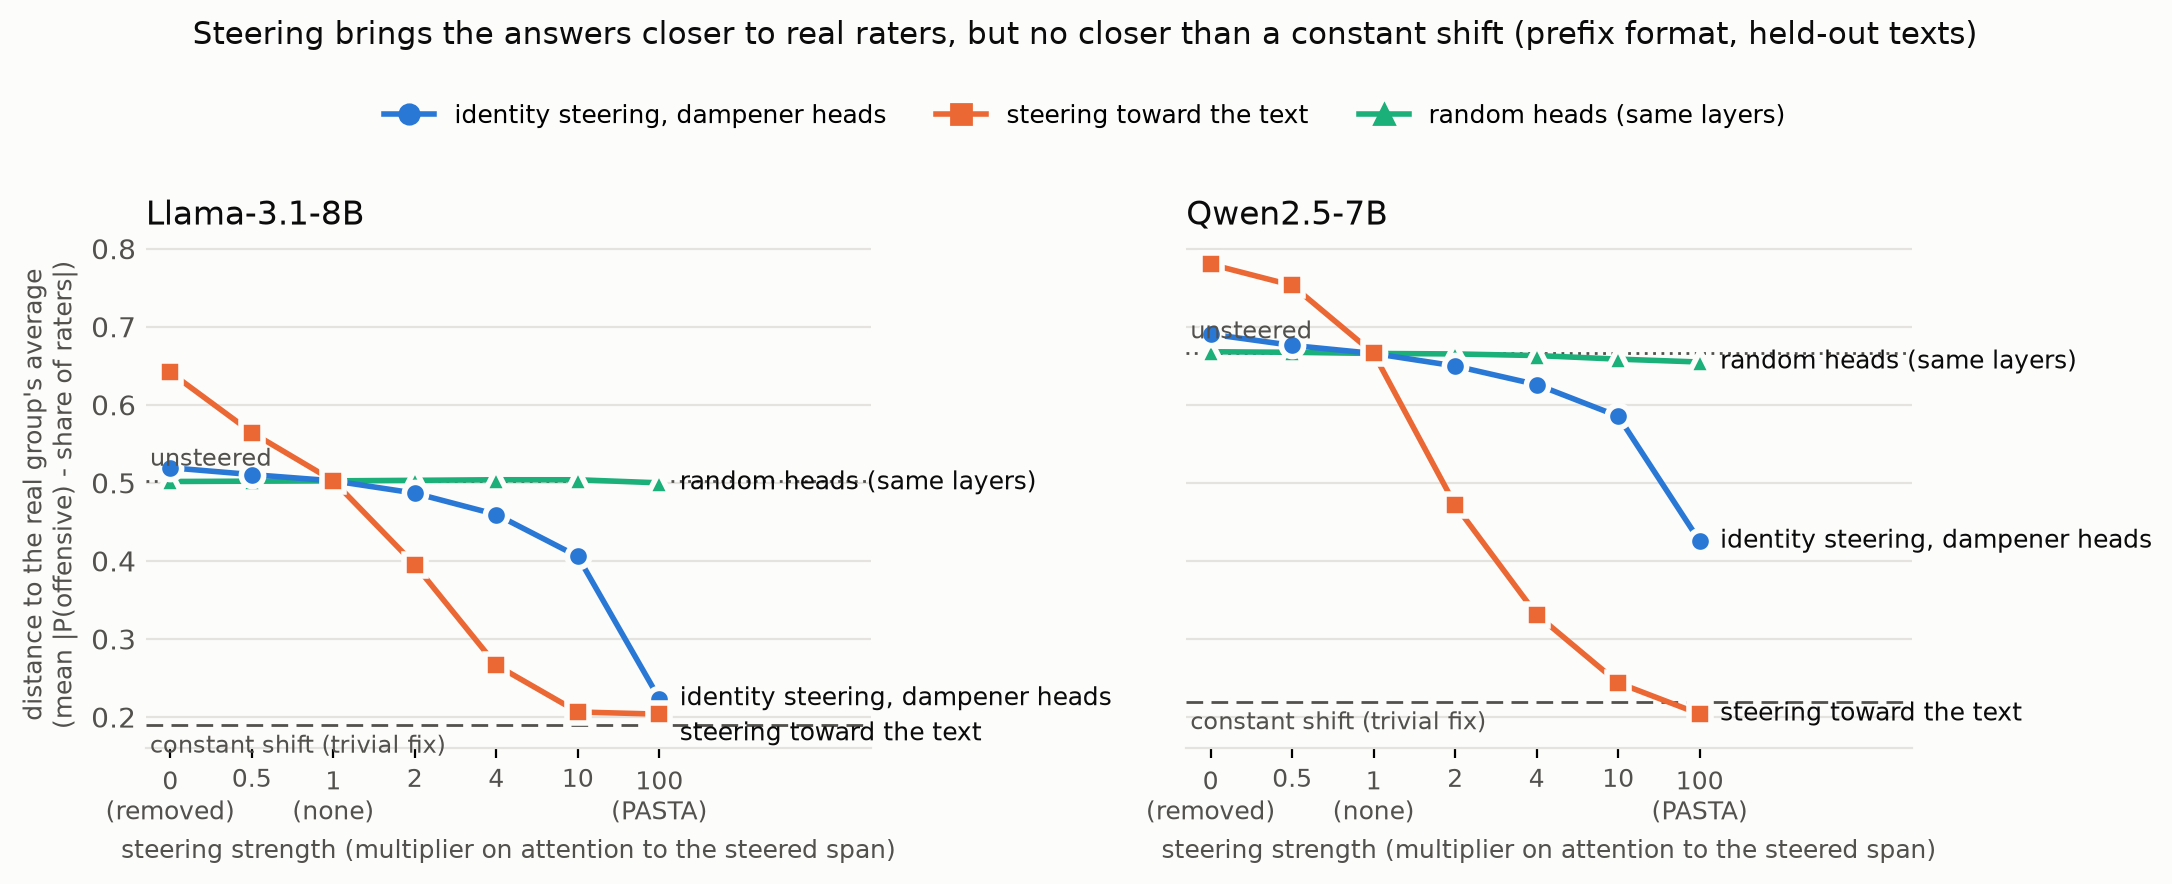
\includegraphics[width=\linewidth]{v3/steering_dose_response.png}
  \caption{Distance to the real group's average rating as a function of steering strength
    (\variant{prefix}, held-out texts). \fillin{Finish caption.}}
  \label{fig:dose-response}
\end{figure}

% ---------------------------------------------------------------------
\subsection{What each method actually does}
\label{sec:steering:methods}
% - Text steering: -5 to -6 log-odds on every prompt incl. unframed; flags
%   0-3% of texts; ranking drops (Llama Spearman 0.13 -> 0.03).
% - Dampeners (Llama): regions -2.5, placebos +1.7, place names +0.6;
%   ranking kept (0.15 -> 0.18); flagged 75% -> 24%. Cleanest
%   identity-specific intervention. Qwen: regions -5.0, placebos -1.5,
%   place -3.4 (partly specific). Not in target.
% - Amplifiers: Qwen regions +4.1, distance +0.09; Llama -0.1.
% - Gender / religion: region dampeners move them much less (-0.7, -0.5).
% - Activation steering: Llama regions -1.4, placebos unchanged; Qwen ~0.
\fillin{Per-method analysis: specificity, ranking, flag rate.}

% Optional table: change in log-odds for region / placebo / place under
% each method (from steering_summary.csv).

% ---------------------------------------------------------------------
\subsection{Alignment versus calibration}
\label{sec:steering:calibration}
% - Relative alignment under steering: rho -0.04 to +0.03 everywhere.
% - Calibrated comparison (table below): after the same constant shift,
%   framing adds nothing (Llama) or hurts (Qwen); predicting each group
%   with the all-raters share is twice as close (0.10).
\fillin{Separating calibration from alignment.}

\begin{table}[t]
  \centering
  \caption{Distance to the real group's share before and after the same constant shift
    (fitted on one half of the texts, evaluated on the other).}
  \label{tab:calibrated}
  \src{v3\_identity\_vs\_baseline.md §1}
  \begin{tabular}{lcccc}
    \toprule
    & \multicolumn{2}{c}{\llamashort} & \multicolumn{2}{c}{\qwenshort} \\
    \cmidrule(lr){2-3}\cmidrule(lr){4-5}
                                       & \variant{prefix} & \variant{infix} & \variant{prefix} & \variant{infix} \\
    \midrule
    unframed, raw                      & 0.34 & 0.34 & 0.42 & 0.42 \\
    framed, raw                        & 0.50 & 0.49 & 0.67 & 0.58 \\
    unframed + constant shift          & 0.19 & 0.20 & 0.20 & 0.20 \\
    framed + constant shift            & 0.19 & 0.19 & 0.24 & 0.23 \\
    dampener-steered + constant shift  & 0.17 & 0.19 & 0.22 & 0.22 \\
    \midrule
    all raters' share as prediction    & \textbf{0.10} & \textbf{0.10} & \textbf{0.10} & \textbf{0.10} \\
    \bottomrule
  \end{tabular}
\end{table}

% =====================================================================
%  7 Results IV: is there a group signal to align with?
%  Sources: reports/v3_identity_vs_baseline.md 2, 3, 4, 6.
%  This section explains WHY no method creates alignment.
% =====================================================================
\section{Results IV: Is There a Group Signal to Align With?}
\label{sec:groupsignal}

% ---------------------------------------------------------------------
\subsection{Text-by-text group differences}
\label{sec:groupsignal:items}
% Method: split each text's raters into two disjoint random halves,
% compute the group gap (group share - rest share) in each half, correlate.
% Result: about 0 for every group, same as random pseudo-groups; faint
% signal for Sinosphere and Sub-Saharan Africa. Partly a sample-size
% limit (2-7 raters per region and text).
\fillin{Split-half reliability of item-level group gaps.}

\begin{table}[t]
  \centering
  \caption{Reliability of per-text group gaps: Spearman correlation between two disjoint halves
    of each group's raters.}
  \label{tab:reliability}
  \src{v3\_identity\_vs\_baseline.md §2}
  \begin{tabular}{lrcc}
    \toprule
    group & texts & mean $|$gap$|$ & split-half $\rho$ \\
    \midrule
    Arab Culture           & \num{1041} & 0.147 & 0.00 \\
    Indian Cultural Sphere & \num{1141} & 0.148 & 0.01 \\
    Latin America          & \num{1058} & 0.151 & 0.02 \\
    North America          & \num{1014} & 0.138 & 0.05 \\
    Oceania                & \num{1016} & 0.137 & 0.03 \\
    Sinosphere             & \num{1242} & 0.161 & 0.10 \\
    Sub-Saharan Africa     & \num{1039} & 0.163 & 0.11 \\
    Western Europe         & \num{1039} & 0.135 & 0.01 \\
    man                    & \num{3297} & 0.129 & 0.01 \\
    woman                  & \num{3321} & 0.128 & 0.00 \\
    \midrule
    random pseudo-group, 1/8 & \num{1562} & 0.157 & 0.02 \\
    random pseudo-group, 1/2 & \num{3258} & 0.130 & 0.02 \\
    \bottomrule
  \end{tabular}
\end{table}

% ---------------------------------------------------------------------
\subsection{Average group offsets}
\label{sec:groupsignal:offsets}
% Regions differ on average (p = 1e-37): Arab Culture +6.6 points,
% Latin America +5.6, Sub-Saharan Africa +2.3, Indian Cultural Sphere
% +1.9, Western Europe -2.0, North America -2.5, Sinosphere -5.6,
% Oceania -6.5. Gender does not (-0.5 / +0.6, p = 0.06).
% Llama gets the order right (rho 0.81, n = 8) with twice the spread;
% Qwen 0.05.
\fillin{Average regional strictness and whether the models reproduce it.}

\begin{figure}[t]
  \centering
  \placeholderfig{Real regional offsets (points) vs each model's region effect, 8 regions,
    one panel per model.}
  \caption{\fillin{Caption.}}
  \label{fig:offsets}
\end{figure}

% ---------------------------------------------------------------------
\subsection{Moral foundations and within-group disagreement}
\label{sec:groupsignal:moral}
% Median splits on each MFQ-2 foundation: same pattern (split-half 0.00
% to 0.07; offsets up to +5.6 points for high care).
% Within-region entropy 0.64 vs 0.80 among all raters of a text: most
% disagreement stays inside a region.
% Consequence: a moral-values framing experiment would likely repeat the
% demographic result, so it was not run.
\fillin{Moral-foundation groups and within-group disagreement.}

\begin{table}[t]
  \centering
  \caption{Moral-foundation groups (median split): reliability of per-text gaps and average offset
    (high minus low half, Mann--Whitney).}
  \label{tab:moral}
  \src{v3\_identity\_vs\_baseline.md §6}
  \begin{tabular}{lrcrr}
    \toprule
    split & texts & split-half $\rho$ & offset (points) & $p$ \\
    \midrule
    high care            & \num{3279} & 0.02 & $+5.6$ & $7\times10^{-18}$ \\
    high equality        & \num{3221} & 0.05 & $+2.1$ & $8\times10^{-3}$ \\
    high proportionality & \num{3146} & 0.00 & $+2.6$ & $2\times10^{-4}$ \\
    high authority       & \num{3141} & 0.06 & $+3.8$ & $2\times10^{-8}$ \\
    high loyalty         & \num{3092} & 0.01 & $+3.7$ & $3\times10^{-7}$ \\
    high purity          & \num{3341} & 0.07 & $+2.9$ & $8\times10^{-5}$ \\
    woman vs rest        & \num{3321} & 0.00 & $+1.3$ & 0.05 \\
    \midrule
    random half (null)   & \num{3258} & 0.02 & $-0.1$ & 0.9 \\
    \bottomrule
  \end{tabular}
\end{table}

% =====================================================================
%  8 Discussion
%  Sources: reports/v3_runC_results.md 5-6, reports/v3_identity_vs_baseline.md,
%  CLAUDE.md section 2 (story), the "honest limits" in
%  reports/proposal_sketch.md section 7.
% =====================================================================
\section{Discussion}
\label{sec:discussion}

\subsection{A model-made group effect}
% Answer RQ1 and RQ2 together: the identity changes the answer (region),
% partly via the place name; the change is not what real groups do.
% Framing moves models away from every group; Llama reproduces the
% direction of regional offsets but exaggerates them (stereotype-like?).
\fillin{Interpretation of the behavioural results.}

\subsection{Calibration is not alignment}
% Why the supervisor's criterion can be met by a constant shift; what a
% better criterion would need (ranking, relative alignment, flag rate,
% soft-label metrics). The Llama dampener heads as the constructive
% result: "removes an identity bias", not "thinks like the group".
\fillin{Interpretation of the steering results.}

\subsection{What the data can and cannot support}
% No reliable item-level group signal in D3CODE (demographic or moral);
% disagreement is mostly within groups. So "make the model act like
% group X" has no item-level target here. Links: Hu & Collier (variance
% explained < 10%), perspectivism literature.
\fillin{Implications of the group-signal analysis.}

\subsection{Implications for LLM-based moderation}
% Over-flagging (recall 0.99, precision 0.26) as the practical issue;
% persona prompts make it worse; threshold / calibration matters more
% than personas; borderline texts.
\fillin{Practical implications.}

\subsection{Lessons for interpretability}
% Attention patterns are a poor guide to causal heads (overlap barely
% above chance); item-level significance under strong single-head
% steering is meaningless without matched nulls; information reaches
% the answer via intermediate tokens.
\fillin{Methodological lessons.}

\subsection{Limitations}
\label{sec:limitations}
% - One dataset, English only, two 7-8B open models, one prompt family,
%   single 0/1 answer token.
% - 500 borderline texts (band filter): results describe borderline
%   texts, not easy ones.
% - Small rater groups per text (>= 4): noisy group shares.
% - Only 2 phrases for gender, religion and identity: low power.
% - Steering strength 100 is extreme; batched bf16 noise up to ~0.5
%   log-odds (handled by within-batch comparisons).
% - Constant shift needs labelled data too.
% - Place controls and steering only for 4 of 8 regions.
\fillin{Limitations.}

\subsection{Ethical considerations}
% Persona prompting can reproduce stereotypes (Llama's exaggerated
% regional offsets); risks of "simulating" groups; D3CODE consent and
% licence; offensive example texts in the thesis (content warning?).
\fillin{Ethics statement.}

% =====================================================================
%  9 Conclusion
%  One paragraph answering RQ1-RQ3 directly, one on future work.
%  Story line (CLAUDE.md section 2): demographic prompting injects a
%  model-made group effect instead of recovering real group perspectives;
%  attention steering can locate and switch off that effect, but cannot
%  create alignment where the data has almost no group-specific signal.
% =====================================================================
\section{Conclusion}
\label{sec:conclusion}

\fillin{Answers to RQ1, RQ2, RQ3.}

% Future work ideas: datasets with more raters per group and text;
% profiling heads against group ratings directly; soft-label targets;
% multilingual data; larger models; per-condition F1 on all texts.
\fillin{Future work.}


\clearpage
\printbibliography[heading=bibintoc]

\clearpage
\appendix
% =====================================================================
%  Appendix A: pilot studies (v1)
%  Sources: reports/attention_probing_final_report.md,
%  reports/attention_layer_analysis.md, reports/disagreement_*.md,
%  reports/master_table_full_analysis.md, reports/zeroshot_results.md,
%  reports/literature_comparison_report.md. History in CLAUDE.md section 4
%  (phases 1-3). Their numbers are superseded by v2; present them as the
%  studies that shaped the final design.
% =====================================================================
\section{Pilot Studies}
\label{app:pilots}

\subsection{Zero-shot baseline on the seeded sample}
% generate() + parsing, 500 seeded test-split items; D3CODE and MHS;
% over-flagging (Llama F1 0.39, 83% predicted positive vs 20% true).
% Decide whether MHS stays (CLAUDE.md section 10).
\fillin{Zero-shot pilot.}

\subsection{Attention probing and placebo pilots}
% 30-item probing (7 conditions): ~80% sink, content attention 87%
% instruction / 13% text, demographic effect in layers 9-18 (peak 13).
% 6 / 100 / 500-item disagreement and placebo studies: ceiling effect,
% single placebo pushing the other way (signed vs unsigned shifts).
\fillin{Probing and placebo pilots.}

\subsection{Master grid v1 and what changed}
% LRZ block design with per-model item sets (Llama 236, Qwen 64).
% Problems fixed in v2 (table below).
\fillin{v1 grid.}

\begin{table}[h]
  \centering
  \small
  \caption{Lessons from the pilots and the design change each one led to.}
  \label{tab:lessons}
  \begin{tabularx}{\linewidth}{XX}
    \toprule
    pilot observation & change in the final design \\
    \midrule
    effects shrink for texts near $\pyes=0$ or 1 (ceiling)  & baseline band $[0.02, 0.98]$ for both models \\
    a single placebo behaved oddly                          & pool of 8 placebos, 2 per length \\
    phrase length drives attention and shifts               & exact token matching; length-adjusted null \\
    different item sets per model                           & one shared list of 500 texts \\
    bf16 output logits round \pyes{}                        & fp32 decision logits \\
    identity phrase found inside the item text              & span search from the end, overlap check \\
    \bottomrule
  \end{tabularx}
\end{table}

% =====================================================================
%  Appendix B: exact prompts and conditions
%  Source of truth: S/master_grid.py (build_content, CONDITIONS,
%  SENTENCE_TEMPLATES, ELABORATION, PERSPECTIVE). Copy strings from there.
% =====================================================================
\section{Prompts and Conditions}
\label{app:prompts}

All prompts are wrapped in each model's chat template as a single user turn.
\fillin{System prompt? (check: none / default of the chat template).}

\noindent\textbf{Unframed.}
\begin{promptbox}
Text: "\{text\}"\\
Is this text offensive? Answer with only 0 (no) or 1 (yes).
\end{promptbox}

\noindent\textbf{\variant{prefix} (example: \cond{someone from Western Europe}).}
\begin{promptbox}
You are someone from Western Europe. Text: "\{text\}"\\
Is this text offensive? Answer with only 0 (no) or 1 (yes).
\end{promptbox}

\noindent\textbf{\variant{infix}.}
\begin{promptbox}
Text: "\{text\}"\\
You are someone from Western Europe. Is this text offensive? Answer with only 0 (no) or 1 (yes).
\end{promptbox}

\noindent\textbf{\variant{embedded}.}
\begin{promptbox}
Text: "\{text\}"\\
As someone from Western Europe, is this text offensive? Answer with only 0 (no) or 1 (yes).
\end{promptbox}

\noindent\textbf{\variant{target}.}
\begin{promptbox}
Text: "\{text\}"\\
Do you think this text is offensive for someone from Western Europe? Answer with only 0 (no) or 1 (yes).
\end{promptbox}

\noindent\textbf{\variant{context\_long}.}
\begin{promptbox}
You are someone from Western Europe. Your background and everyday experience shape how you read
things. Answer from that perspective. Text: "\{text\}"\\
Is this text offensive? Answer with only 0 (no) or 1 (yes).
\end{promptbox}

\fillin{Add the remaining formats if wanted; add the token-length table
(S/results/v2/master\_grid/matching\_*).}

% =====================================================================
%  Appendix C: additional results
%  Candidates: per-region effects (v2 report section 2), all 10 formats
%  of the identity-vs-placebo test (behaviour_axis_tests.csv), paraphrase
%  consistency, moderators (category, baseline, entropy), cross-model
%  agreement, full steering tables (steering_summary.csv), dose-response
%  for infix and target, random-head distributions.
% =====================================================================
\section{Additional Results}
\label{app:results}

\begin{table}[h]
  \centering
  \caption{Single regions under \variant{prefix} against a content-free phrase of the same length
    (log-odds; $^\ast$\,$p<0.05$ at the phrase level).}
  \label{tab:regions}
  \src{v2\_behavioural\_analysis.md §2}
  \begin{tabular}{lrr}
    \toprule
    region & \llamashort & \qwenshort \\
    \midrule
    Sub-Saharan Africa     & $+2.97^\ast$ & $+5.56^\ast$ \\
    Arab Culture           & $+1.99^\ast$ & $+3.98^\ast$ \\
    Sinosphere             & $+1.36^\ast$ & $+3.92^\ast$ \\
    Indian Cultural Sphere & $+1.51^\ast$ & $+3.68^\ast$ \\
    Latin America          & $+2.17^\ast$ & $+1.26$ \\
    Western Europe         & $+1.27^\ast$ & $+2.29$ \\
    Oceania                & $+1.18^\ast$ & $+2.34$ \\
    North America          & $+0.98$      & $+1.71$ \\
    \bottomrule
  \end{tabular}
\end{table}

\fillin{More tables and figures as needed.}

% =====================================================================
%  Appendix D: reproducibility
%  Sources: CLAUDE.md sections 5, 6 and 12; reports/coma_runbook_v2.md.
% =====================================================================
\section{Reproducibility}
\label{app:repro}

\paragraph{Compute.} \fillin{COMA cluster, NVIDIA H200, GPU hours per run (A, B, C).}

\paragraph{Software.} Python 3.12, PyTorch 2.14.1 (CUDA 13), Transformers 5.14.1.
\fillin{Model revisions / commit hashes from the HF cache.}

\paragraph{Code and data.} \fillin{Repository link; which script produces which table
(CLAUDE.md section 5).}

\paragraph{Determinism.} Repeated runs give identical outputs (noise check: 0);
batched and single runs differ by up to about 0.5 log-odds because of bf16 and padding,
so steered and unsteered prompts are always compared within the same batch.

\paragraph{Use of AI assistants.} \fillin{State how AI tools were used (code, analysis,
writing), as required by your examination regulations.}


\clearpage
% ---------------------------------------------------------------------
%  Declaration of authorship. Most universities prescribe the exact
%  wording (often in German: "Eidesstattliche Erklaerung"). Replace this
%  text with the official version from your examination office.
% ---------------------------------------------------------------------
\section*{Declaration of Authorship}
\addcontentsline{toc}{section}{Declaration of Authorship}

I hereby declare that I have written this thesis independently and have not
used any sources or aids other than those indicated. All passages taken
literally or in spirit from other sources are marked as such.
\fillin{Replace with the official wording, including the required statement
on the use of AI tools.}

\vspace{2cm}
\noindent\fillin{Place, date} \hfill \rule{6cm}{0.4pt}\\
\hspace*{\fill}Tarik Akinci


\end{document}
